Рассмотрим вышеупомянутые алгоритмы сортировки. Для удобства изложения сути алгоритмов, будем рассматривать сортировку по неубыванию. Алгоритмы сортировки других порядков могут быть получены заменой условия сравнения.

\section{Сортировка пузырьком}
Алгоритм сортировки пузырьком основывается на следующем действии. Массив проссматривается от 0 до N-2 элемента, и в случае, если текущий элемент массива больше следующего, они меняются местами. Таким образом, после первого прохода в конце массива окажется максимальный элемент, после второго - два максимальных, и так далее до полного упорядочивания массива.

Схема алгоритма приведена на рисунке 2.1.
\begin{figure}[h]
	\begin{center}
		{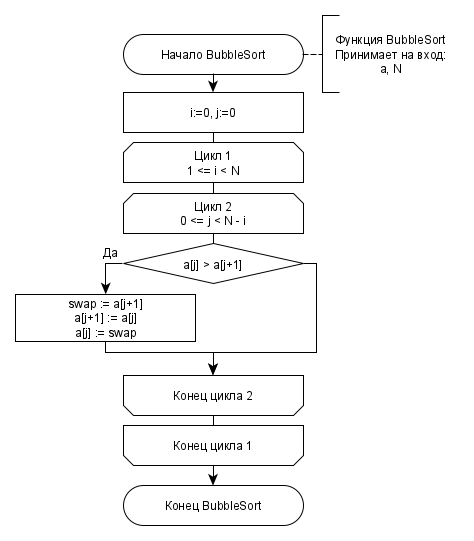
\includegraphics[height=20cm, width = 17cm]{Bubble}}
		\caption{Сортировка пузырьком}
	\end{center}
\end{figure}


\section{Поразрядная сортировка}
Цель алгоритма заключается в реализации трудоёмкости, линейно зависящей от размера массива. Упорядоченнсть достигается последовательной сортировкой по значению разрядов (в порядке от меньшего разряда к большему). Алгоритм применим к массиву, состоящему из целых положительных чисел или иных значений, которые м.б. спроецированы на множетво положительных чисел \cite{Korman}. 

Будем считать, что максимальное число в массиве состоит из K разрядов. В случае, если массив содержит целыйе отрицательные числа, то перед сортировкой все числа должны быть увеличены на модуль минимального числа, а после сортировки уменьшены.

Схема алгоритма приведена на рисунках 2.2. и 2.3.
\begin{figure}[h]
	\begin{center}
		{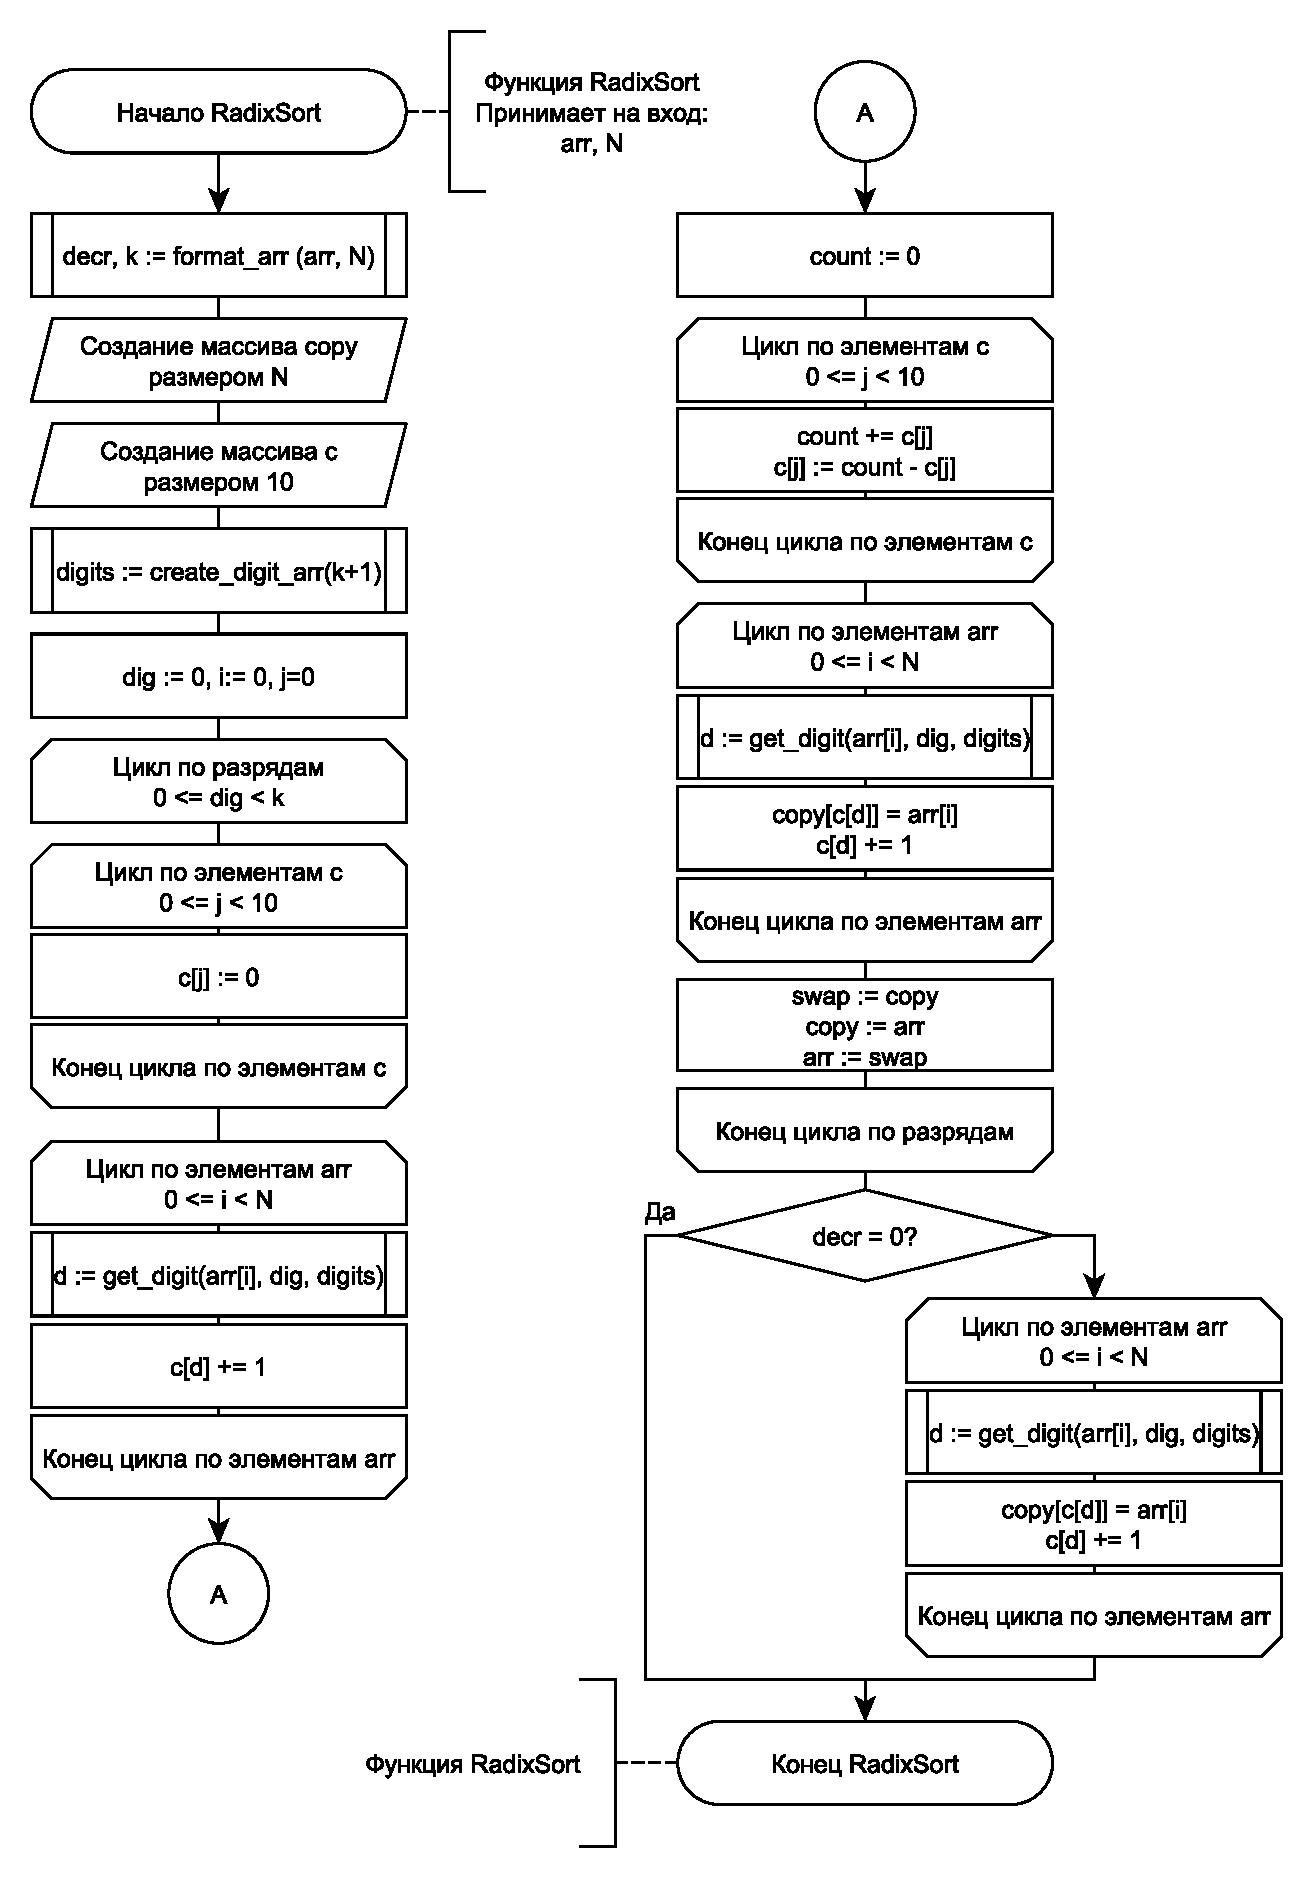
\includegraphics[height=20cm]{Radix1}}
		\caption{Поразрядная сортировка (часть 1)}
	\end{center}
\end{figure}

\begin{figure}[h]
	\begin{center}
		{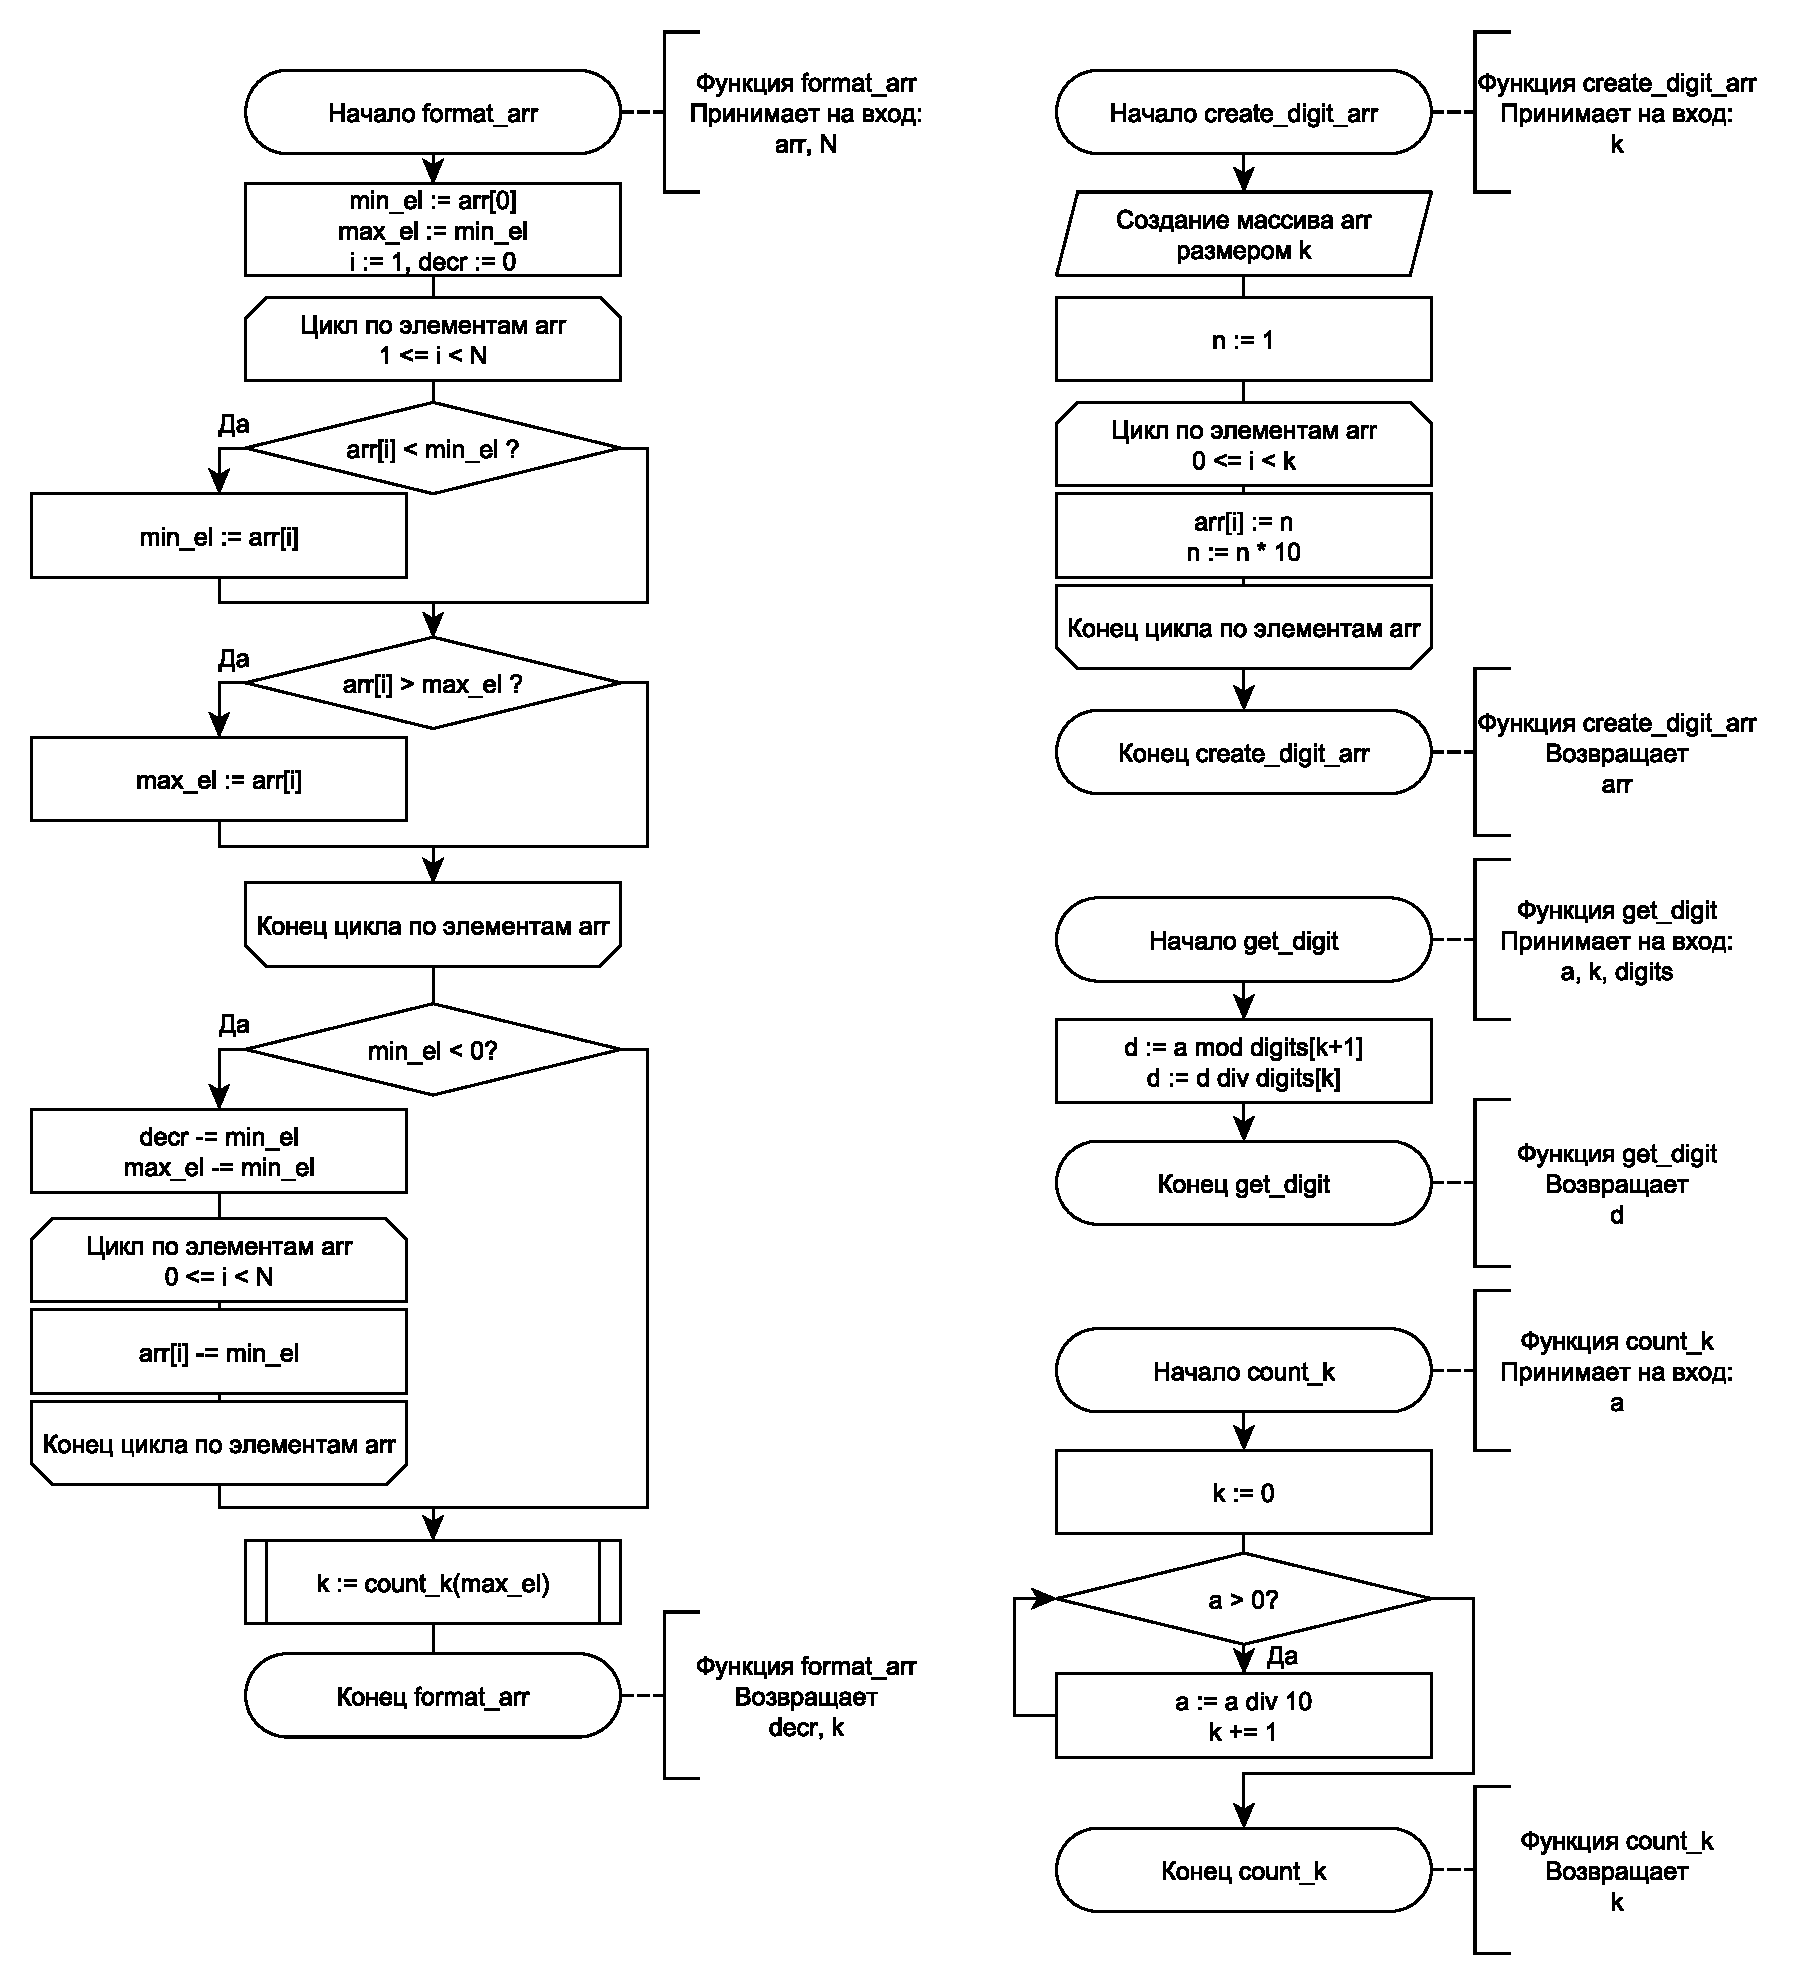
\includegraphics[width = 17cm]{Radix2}}
		\caption{Поразрядная сортировка (часть 2)}
	\end{center}
\end{figure}


\section{Сортировка слиянием}
Идея алгоритма заключается в том, что достаточно эффективно производится операция слияния (т.е. создания из двух массивов одного) при условии, что оба сливаемых массива уже упорядочены. Алгоритм разбивает массив на два подмассива, после чего применяет к ним ту же операцию, до тех пор, пока длина массива не станет меньше 3. После завершения сортировки подмассивов производится построение упорядоченного массива их слиянием.

Схема алгоритма приведена на рисунке 2.4.
\begin{figure}[h]
	\begin{center}
		{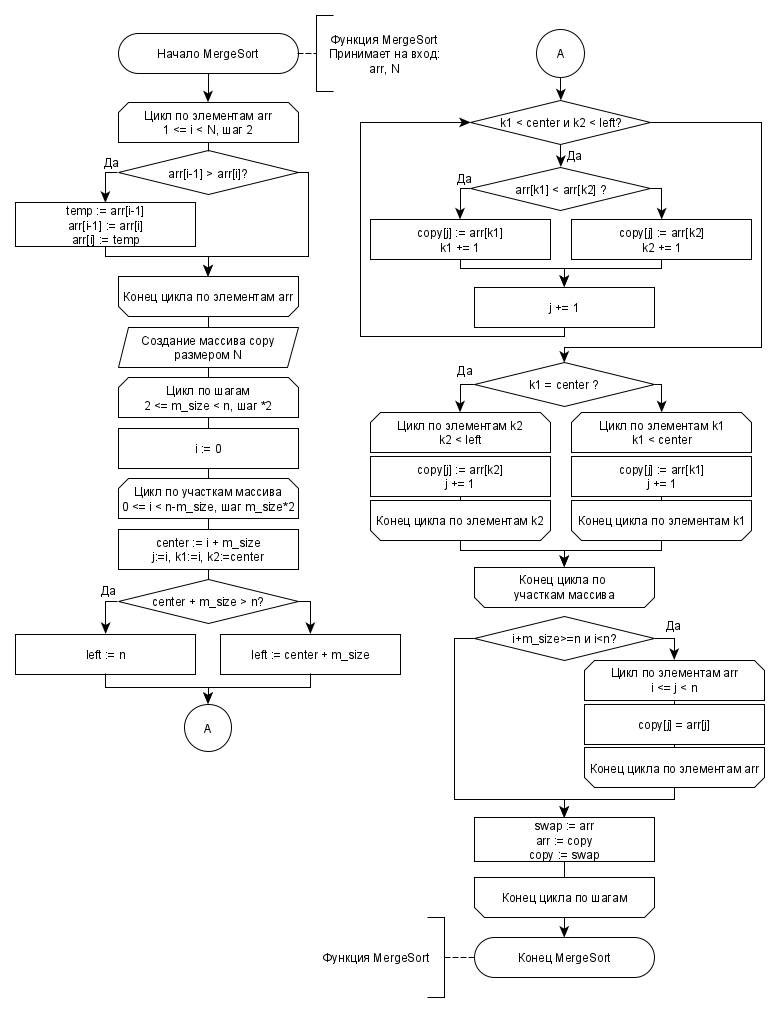
\includegraphics[height=20cm]{Merge}}
		\caption{Сортировка слиянием}
	\end{center}
\end{figure}


\section{Требования к программному обеспечению}
Для полноценной проверки и оценки алгоритмов необходимо выполнить следующее.
\begin{enumerate}
	\item Обеспечить возможность консольного ввода массива и выбора алгоритма сортировки. Программа должна вывести отсортированный массив.
	\item Реализовать функцию замера процессорного времени, затраченного функцией. Для этого также создать возможность ввода размера массива, на котором будет выполнен замер.
\end{enumerate}


\section{Заготовки тестов}
При проверке алгоритмов необходимо будет использовать следующие классы тестов:
\begin{itemize}
	\item массив размером 1;
	\item массив одинаковых элементов;
	\item упорядоченный и обратно упорядоченный массив.
\end{itemize}

\section*{Вывод}
Результатом конструкторской части стало схематическое описание алгоритмов сортировок, задание требований к программному обеспечению и к системе тестов.

